% !TEX root = ../main.tex

% 中英标题：\chapter{中文标题}[英文标题]
\chapter{绪论}[Introduction]

\section{本文研究背景}
近年来，随着互联网的快速发展和数据规模的急剧膨胀，现实世界的信息量呈现出指数级增长的趋势。用户在享受信息便利的同时，也面临着“信息过载”的问题，即如何在海量数据中高效地筛选出符合个人兴趣和需求的内容，已成为当前研究和产业界的核心挑战之一。推荐系统（Recommender System, RS）正是在这一背景下应运而生，它通过分析用户与物品之间的历史交互关系来学习用户与物品的表示，从而为用户提供个性化内容推荐\cite{中文推荐算法综述2009, gao2022graph-survey,zhou2023comprehensive}。推荐系统如今已成为互联网产品的重要组成部分，被广泛应用于视频平台（如 YouTube、抖音）、音乐平台（如 QQ 音乐、网易云音乐）以及电商平台（如淘宝、拼多多、京东）等，为用户带来便利体验的同时也为企业创造了显著的商业价值。

推荐系统的发展大致经历了从基于相似度的协同过滤（Collaborative Filtering, CF）\cite{collaboratives2025survey}，到基于深度学习的表示学习方法\cite{zhou2023comprehensive}，再到近年来基于图神经网络（Graph Neural Network, GNN）\cite{gao2022graph-survey}的阶段。协同过滤通过度量用户或物品间的相似性实现推荐，而深度学习方法利用神经网络提升了表示能力。近年来，GNN 被广泛应用于推荐系统中，能够在用户–物品二部图上建模高阶关系，通过消息传递机制捕捉潜在的交互模式，从而显著提升推荐性能。

在实际的电商场景中，不同平台的用户行为模式呈现显著差异。例如，淘宝具有多场景、多触点的推荐链路，用户浏览行为丰富但意图跨度较大；拼多多用户的交互频率较高，但弱意图点击占比更大、噪声比例更高；京东的行为密度相对较低，但购买类行为更能直接反映用户的明确偏好。这些平台在用户行为密度、意图强度与噪声比例方面的结构性差异，导致行为数据在语义和质量上存在显著不一致性，也使得推荐模型在不同平台上的行为建模面临更高挑战。

值得注意的是，现有的多数图神经网络推荐方法仍仅基于用户的单一目标行为（如购买）进行建模\cite{he2020lightgcn, fan2023graphDA, wang2019NGCF}。这一简化假设在真实平台的复杂交互场景下存在明显局限。事实上，用户往往会对同一物品产生多种行为\cite{chen2021GHCF, gu2022S-MBRec}，如浏览、收藏、加购、购买等。这些行为反映了从浅层兴趣到深层意图的渐进过程，蕴含着更丰富的语义信息。为缓解数据稀疏问题并增强模型的表达能力，多行为推荐（Multi-Behavior Recommendation, MBR）通过引入辅助行为来扩充目标行为的有效信号。

但与此同时，引入辅助行为的同时也带来了大量噪声行为。由于弱意图行为（如浏览、随手点击）的语义更弱且不可控，这些行为容易偏离用户的真实兴趣。如果直接将其纳入建模，将干扰模型的偏好学习过程，甚至导致推荐结果偏移。因此，如何有效识别并抑制多源行为中的噪声影响，成为当前多行为推荐研究面临的核心挑战之一。

\section{本文研究目的}
针对目前多行为推荐系统在去噪方面的研究不足，本文拟提出一种基于图神经网络的多行为去噪推荐模型。该模型通过在多行为图结构中引入噪声建模与关系加权机制，实现对多源行为的联合学习与鲁棒推荐。本文的研究目标在于提升推荐系统在复杂行为场景下的准确性与鲁棒性，同时为多行为数据的统一建模与泛化能力提供新的思路，从而推动推荐系统在真实环境中的稳定性与应用效果。

\section{国内外相关研究概述}

\subsection{基于图神经网络的推荐算法研究现状}
近年来，图神经网络凭借其在处理图结构化数据方面的强大建模能力，已成为推荐系统领域的重要研究方向。推荐系统的核心任务是基于用户的历史行为预测其未来的兴趣偏好，而用户与物品之间的交互关系可以自然地建模为图结构，这使得 GNN 在该场景中展现出独特优势。

GNN 能够在用户–物品二部图上建模高阶交互关系\cite{ying2018Pinsage}。其中，用户和物品分别作为节点，交互行为作为边，通过消息传递与聚合机制，模型能够捕获潜在的关系模式，从而学习到更具表达力的用户与物品表示。此外，GNN 还可进一步融合外部信息，例如用户的社交关系\cite{wu2019Social} 和物品的知识图谱\cite{wang2019Knowlegde-Graph}，以构建统一的表示学习框架，更全面地刻画推荐系统中的异构数据特征。

图神经网络在推荐系统中的发展呈现出“结构简化”与“学习范式增强”双轨并进的趋势。早期工作 NGCF\cite{wang2019NGCF} 首次将协同过滤信号嵌入图神经网络的消息传递过程，通过多层邻居聚合捕获高阶交互关系，但其引入的非线性变换导致计算复杂度高且易引发过平滑问题。针对此局限，LightGCN\cite{he2020lightgcn} 通过移除非线性激活与特征变换层，仅保留邻居聚合与层间加权操作，在显著降低计算开销的同时保持了优异性能，验证了简洁图卷积结构在推荐任务中的有效性与鲁棒性。为进一步提升模型泛化能力，研究者将自监督对比学习引入图推荐框架：SGL\cite{wu2021SGL} 基于图结构数据增强构建多视角表示，通过拉近同一节点在不同视角下的嵌入距离增强表征一致性；而 SimGCL\cite{liu2024simgcl} 则进一步简化流程，摒弃复杂的数据增强操作，转而通过在嵌入空间施加可控噪声扰动实现对比学习，以更轻量的结构取得相当甚至更优的效果。这一系列工作表明，通过结构精简与自监督机制的协同设计，图神经网络推荐模型在效率、稳定性与泛化能力方面实现了系统性提升，为后续研究提供了清晰的技术路径与理论启示。

综上，基于图神经网络的推荐研究已取得显著进展，但在多行为建模方面仍存在不足。为进一步挖掘用户偏好的多层次特征，研究者开始探索基于图神经网络的多行为推荐方法，这将在下一节中详细介绍。

\subsection{基于图神经网络的多行为推荐研究现状}
传统的推荐模型通常仅利用单一类型的用户–物品交互行为进行建模，因此容易面临数据稀疏和冷启动等问题。多行为推荐通过引入多种用户–物品交互类型（例如浏览、收藏、加入购物车等），为缓解上述问题提供了有效的解决思路\cite{RJXB202405021, JSJY20240626002, HNSF202304008, ZDZC202310007}。在多行为场景中，如何实现辅助行为（如浏览、收藏、加购）与目标行为（如购买）之间的有效信息融合，一直是学术界关注的研究重点。相关研究主要聚焦于探索不同行为之间的语义关联与交互机制，以提升目标行为的预测性能。图 1-1 展示了多行为推荐中典型的多种行为数据形式及其对应的推荐目标。

\begin{figure}[h]
\centering
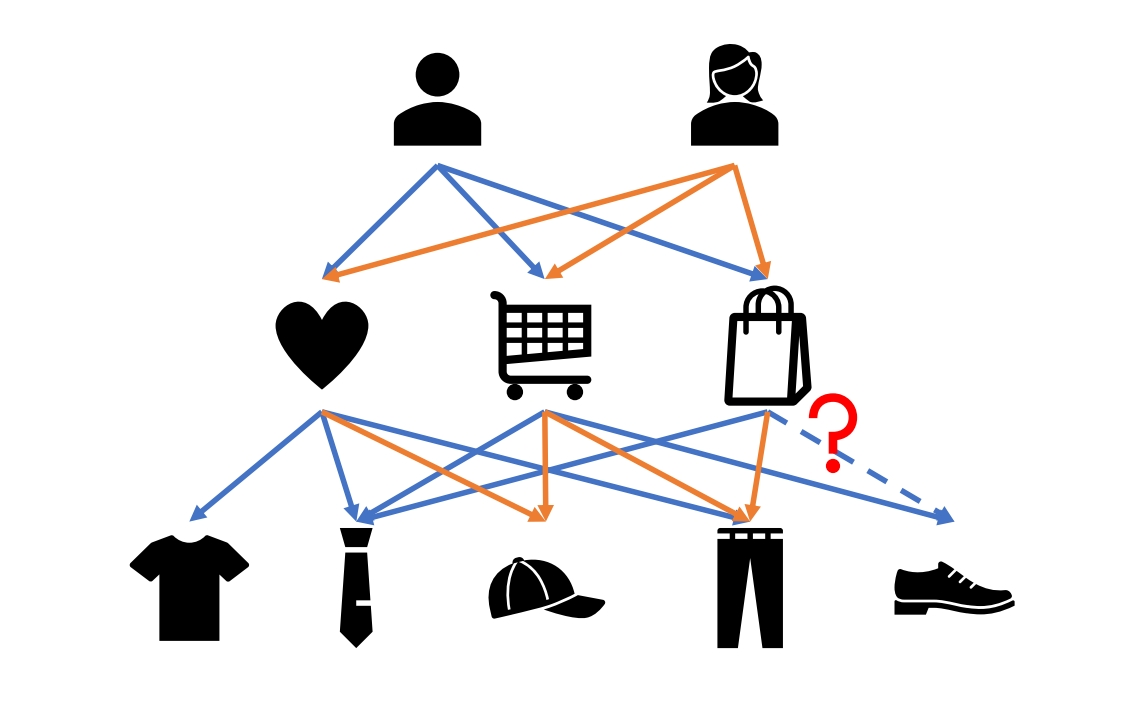
\includegraphics[width = 0.75\textwidth]{figures/Multi-Behavior-U-I.png}
\caption{多行为推荐的数据形式\cite{gao2022graph-survey}}
\label{fig:Multi-Behavior-U-I}
\end{figure}

在多行为推荐研究中，如何有效融合异构行为信号、建模行为间复杂关系并提升模型鲁棒性，成为持续演进的核心议题。Jin 等人 \cite{jin2020MBGCN} 提出的 MBGCN 模型率先构建统一异构图结构，通过用户–物品二部图学习行为交互贡献，并在物品–物品共同交互图上建模行为语义相关性，实现多行为信号的互补融合，但其在噪声行为处理与行为依赖建模方面仍显不足。针对行为间依赖关系与用户行为模式差异性问题，Xia 等人 \cite{xia2021MB-GMN} 引入元学习框架，将不同行为视为独立任务，通过动态调整图神经网络参数实现跨行为知识迁移，显著增强了模型对多样化用户行为的适应能力，然而训练复杂度较高且对参数初始化较为敏感。为挖掘行为共性以缓解监督信号稀疏，Gu 等人 \cite{gu2022S-MBRec} 设计 S-MBRec 模型，借助自监督学习最大化目标行为与辅助行为嵌入的一致性，在提升信号利用率的同时减少冗余，但对噪声行为的鲁棒性仍有提升空间。进一步地，Cheng 等人 \cite{cheng2023cascading} 观察到多行为常呈现顺序性与因果依赖，提出 Cascading GCN 模型，通过级联结构将前序行为嵌入传递至后续行为的图卷积层，显式刻画用户兴趣的动态演化过程，但其对预设行为顺序的依赖限制了在非线性行为模式下的适用性。为突破多行为独立建模的局限，Zhang 等人 \cite{zhang2024POGCN} 提出 POGCN 模型，定义行为间的偏序关系并构建加权图结构，在保留层次差异的同时实现全局行为融合，然而该方法仍未充分区分不同行为的信噪差异。在此基础上，Zhang 等人 \cite{zhang2023DPT} 进一步提出 DPT 模型，采用预训练策略对辅助行为交互进行质量评估与噪声过滤，在清洗后的数据上联合训练以提升表示质量，但其去噪机制与多行为关联结构解耦，且未能自适应建模各类行为的噪声比例差异。综上，多行为推荐研究正沿着“结构融合→依赖建模→自监督增强→顺序感知→偏序整合→噪声鲁棒”这一技术脉络持续深化，未来工作需进一步协同优化行为语义建模、动态依赖捕捉与噪声自适应处理能力，以构建更精准、稳健的用户兴趣表征框架。

虽然多行为推荐已取得显著进展，但现有研究大多关注于如何将多种行为信息进行融合，而较少考虑辅助行为中潜在的噪声问题。在实际场景中，诸如点击、浏览、收藏等辅助行为通常成本较低、随意性较强，往往不能准确反映用户的真实兴趣或购买意图，从而引入大量噪声。尽管 DPT 模型\cite{zhang2023DPT} 尝试对辅助行为进行去噪，但其仍沿用单行为推荐中的独立去噪思路，未能充分建模多种行为之间的关联差异。事实上，不同行为对用户偏好的反映程度并不相同，其噪声比例也应具有差异。因此，如何在多行为推荐中有效识别并抑制噪声行为，成为当前研究亟待解决的问题，也促使去噪推荐逐渐成为新的研究方向。

\subsection{去噪推荐算法研究现状}
推荐系统主要依赖于隐式反馈（Implicit Feedback）来学习用户偏好。隐式反馈指用户在与系统交互过程中无需明确表达意图，系统根据用户的行为（如点击、浏览、收藏等）推断其兴趣偏好。与显式反馈（如评分或评论）相比，隐式反馈更易获取且更符合用户的真实行为特征。然而，在实际场景中，隐式反馈往往包含大量噪声样本，如误点击、随机浏览或非兴趣驱动的交互，这些噪声会干扰模型对用户真实偏好的学习，导致推荐性能下降。因此，如何识别并抑制噪声反馈，成为推荐系统研究中的重要问题\cite{JSJY2024S1014}。

在推荐系统的噪声鲁棒性研究中，去噪策略的设计逐步从单点优化走向结构感知与多粒度协同。Wang 等人 \cite{wang2021ADT} 首次提出基于训练动态的自适应去噪框架（ADT），通过监测隐式交互的损失值分布，采用截断或加权策略动态抑制高损失样本的干扰，奠定了“训练信号驱动去噪”的基础范式。然而，该方法未考虑图结构中噪声通过邻域聚合的传播效应。针对此局限，Tian 等人 \cite{tian2022learning-to-denoising} 引入图去噪模块与多样性保持模块：前者优化图拓扑以筛选可靠交互关系，后者联合去噪数据与多样性增强样本进行训练，在抑制全局噪声扩散的同时缓解了过度去噪引发的数据稀疏问题。进一步地，Fan 等人 \cite{fan2023graphDA} 指出交互频次异质性带来的双重挑战——稀疏节点信息不足与密集节点噪声冗余，提出 GraphDA 模型：通过预训练获取节点嵌入，并采用 Top-K 双向增强策略，对稀疏节点进行语义扩充、对高频节点实施精准去噪，有效平衡数据不平衡与噪声干扰。然而，基于瞬时损失的噪声判别易受困难样本干扰，评估稳定性不足。He 等人 \cite{he2024double} 提出 DCF 模型，通过聚合多轮训练迭代的损失轨迹提升样本评估鲁棒性，并创新性地将标记噪声样本重新标注后参与训练，在增强模型抗噪能力的同时避免了有效信息的浪费。近期，Zhang 等人 \cite{zhang2025dembr} 将去噪机制拓展至多行为推荐场景，设计 DeMBR 双层框架：硬去噪层依据多行为嵌入相似度剔除低质量交互；软去噪层则引入语义引导机制，以强表达行为（如购买）的语义信号校准弱表达行为（如点击）的噪声分布。该方法虽显著提升多行为推荐性能，但仍依赖预设行为强度假设，缺乏对噪声比例的动态感知能力。综上，去噪研究已从“单点损失筛选”演进至“图结构优化—频次感知增强—多轮评估稳定—多行为语义协同”的系统化框架，未来需进一步融合自适应噪声建模、行为强度动态校准与图结构演化感知，以构建更具鲁棒性与解释性的推荐系统。

综上所述，现有去噪推荐研究主要聚焦于单行为隐式反馈场景下的噪声识别与抑制，通过损失监测、自适应加权或图结构重构等手段提升模型鲁棒性。然而，在多行为推荐系统中，辅助行为（如浏览、收藏、加购）普遍存在噪声，而相关研究仍较为匮乏。当前方法往往假设所有辅助行为的噪声分布一致，忽略了不同行为在用户偏好反映上的差异性。针对这一问题，本文将从“多行为去噪”的角度出发，探索在图神经网络框架下识别并抑制辅助行为噪声的新方法，以更准确地刻画用户真实兴趣并提升多行为推荐性能。

\subsection{多模态与大模型驱动的推荐研究现状}

\textbf{(1)多模态推荐研究现状}

近年来，研究者开始探索在推荐系统中融合多模态信息，以更全面地理解用户兴趣与物品语义。多模态推荐通过结合文本、图像、音频等内容特征，能够在冷启动与稀疏交互场景下显著提升模型性能。然而，现有多模态推荐方法普遍存在两个主要不足：一是多数模型仅在特征层面进行模态信息的简单融合，未能充分建模不同模态之间的交互与互补关系；二是模态特征中常存在噪声（如图像背景干扰或文本冗余描述），若未加以抑制，可能会削弱模型对用户真实偏好的刻画精度。

在多模态推荐研究中，如何有效挖掘模态内容蕴含的物品关联结构，并协同处理模态噪声与特征冗余，成为提升推荐质量的关键挑战。Zhang 等人提出的 LATTICE 模型 \cite{zhang2021mining} 首次系统构建了多模态隐式关联图谱，为图像、文本等各模态分别建立物品–物品图，并聚合为统一的潜在结构图进行图卷积传播，实现了模态语义与协同信号的有效融合。然而，该模型未显式建模模态间的互补关系，亦缺乏对模态特征中噪声干扰的鲁棒性处理机制。针对图结构效率与交互噪声问题，Zhou 等人 \cite{zhou2023tale} 提出 FREEDOM 模型，在保留 LATTICE 多模态图框架的基础上，通过冻结物品–物品图降低训练开销，并对用户–物品交互图实施剪枝与去噪策略，显著提升了模型稳定性与计算效率；但其仍未深入挖掘模态间的语义互补性，也未对模态内部噪声进行显式建模。为进一步解决多模态图神经网络中的特征冗余与模态噪声耦合问题，Mo 等人 \cite{mo2024multimodal} 提出 MGNM 模型，构建局部–全局协同优化框架：在局部交互层面，引入动态去冗余损失，通过约束特征矩阵与系数矩阵的乘积关系，有效抑制多层传播引发的特征冗余；在全局交互层面，设计模态引导的特征去噪模块，针对性滤除与用户偏好无关的模态噪声，并显式建模模态内部的复杂语义关联。这一技术演进脉络清晰呈现了多模态推荐研究从“多模态图构建”到“结构效率优化”，再到“精细化噪声抑制与冗余控制”的深化过程，为后续融合模态互补性建模与自适应去噪机制的研究提供了重要思路。

总体而言，现有多模态推荐研究在提升模型表达能力和缓解数据稀疏方面取得了显著进展。然而，大多数方法仍主要关注模态内部特征的融合，而缺乏对不同模态间交互与语义互补关系的系统建模。同时，模态特征本身往往存在噪声与冗余信息，若未有效抑制，可能导致推荐结果偏离用户真实偏好。这些局限性为后续将大模型（LLMs）引入推荐系统以实现跨模态语义理解与知识增强提供了新的研究方向。

\textbf{(2)大模型结合推荐研究现状}

近年来，大语言模型（Large Language Models, LLMs）在自然语言处理领域展现出强大的语义理解与推理能力，推动了推荐系统研究的新方向。LLM 在推荐系统中的应用主要集中于特征工程阶段，利用其开放世界知识与逻辑推理能力对原始数据进行后加工与数据增强，以生成语义更丰富的特征或样本，缓解数据稀疏与冷启动问题。然而，现有多模态推荐方法往往忽视模态之间的关联性与模态内部的噪声特征，导致特征融合效果受限。为此，本文引入大语言模型作为语义引导模块，通过深层语义建模与关系补全来显式建模模态间关联，并削弱模态内部噪声，从而实现跨模态信息的语义对齐与高质量特征融合，提升推荐系统的鲁棒性与语义表达能力。

为应对推荐系统中数据稀疏、语义理解不足及噪声干扰等核心挑战，研究者积极探索将预训练语言模型与多模态技术深度融入推荐框架。Wei 等人提出的 LLMRec 模型 \cite{wei2024llmrec} 首次系统性地利用大型语言模型（LLM）的通用知识与推理能力，从自然语言视角对推荐图进行三重增强：强化用户–物品交互边以丰富隐式反馈信号、深化物品节点的语义表征、构建细粒度自然语言用户画像，显著提升了稀疏场景下的语义理解与个性化建模能力。在多模态语义融合方向，Xu 等人 \cite{MMPOI} 针对兴趣点推荐中的模态异构问题，设计统一语义对齐框架：借助 BLIP2 \cite{pmlr-v202-li23q} 将图像内容转化为结构化文本描述，并通过 Sentence-BERT \cite{reimers2019sentence} 统一提取多模态语义表示，有效消解视觉与文本模态间的语义鸿沟，增强内容表达的完整性与一致性。进一步地，Wang 等人 \cite{wang2025unleashing} 提出的 LLaRD 模型将 LLM 的能力延伸至噪声鲁棒性优化，突破传统去噪方法对外部知识或固定假设的依赖，创新性地引入语言先验与链式思维（CoT）推理机制：首先由 LLM 从交互数据中提炼用户偏好语义知识，继而通过逻辑推理显式识别并过滤无关或错误交互，在保留有效信息的同时显著提升模型抗噪能力。上述工作共同勾勒出预训练模型赋能推荐系统的技术演进路径——从图结构语义增强、多模态语义对齐，到基于语言推理的噪声感知与净化，标志着推荐系统正逐步迈向“语义驱动、认知增强”的新阶段，为构建更智能、可解释且鲁棒的下一代推荐框架提供了关键思路。
总体来看，近年来大语言模型（LLMs）在推荐系统中的引入，为缓解数据稀疏、语义不一致及噪声干扰等长期难题提供了新的思路。相关研究表明，LLM 不仅能够利用其开放世界知识和推理能力丰富用户与物品的语义表示，还能在多模态融合与交互建模中发挥语义引导作用。

\subsection{研究概述小结}
在多行为推荐系统中，现有研究主要聚焦于利用多种用户交互行为（如点击、加购、收藏和购买）来缓解数据稀疏问题并提升推荐精度。然而，尽管多行为建模显著改善了用户偏好的捕获能力，现有方法在噪声识别与偏好提取方面仍存在若干不足与挑战：

\textbf{辅助行为噪声问题：} 辅助行为虽能提供额外的用户偏好线索，但其中包含大量与真实兴趣无关的交互，例如偶然点击或临时操作。这类偶然点击通常表现为：与用户长期兴趣模式不一致的短期行为、在相似用户交互中缺乏支持，以及未触发后续高价值行为。在多行为推荐建模中，这类噪声可能在图传播过程中被放大，导致模型学习到的用户偏好偏离真实分布。目前大多方法仍将不同辅助行为视为等价信号，缺乏对行为强度差异与行为内相关性的细粒度建模。为缓解其干扰，本文在后续方法中主要从两个维度识别辅助行为噪声：一是依据不同行为类型的强度差异赋予行为权重，反映其对目标偏好的可信度；二是基于相似用户的局部一致性，通过用户间共同交互模式评估单条行为的可靠性，从而有效过滤低可信度的噪声交互。


\textbf{行为间依赖关系建模不足：} 多行为推荐往往将辅助行为直接与目标行为进行融合，却忽略了行为间的层次与依赖结构。例如，加购行为对购买的促进作用远强于点击行为，若未能显式区分不同行为的影响强度，容易引入跨行为噪声并造成信息混淆。

\textbf{模态特征噪声与异构性问题：} 随着多模态推荐的兴起，视觉、文本等模态特征被广泛用于丰富物品表示。然而，不同模态间存在显著的语义空间差异，而单一模态内部也常含有噪声或冗余信息。若缺乏有效的模态对齐与噪声抑制机制，模态融合反而可能削弱推荐的语义一致性。

\textbf{语义层面真实偏好提取不足：} 当前大多数方法仅依赖结构化交互数据进行建模，忽视了从语义层面理解与提炼用户真实偏好的可能性。由于交互行为背后潜藏着复杂的语义意图，单纯依赖协同信号难以全面刻画用户兴趣。

综上，现有研究在多行为推荐的去噪建模中仍存在结构层与语义层的双重瓶颈。为此，本文分别从\textbf{协同信号层面与语义层面}提出系统性改进：第一，设计基于协同信号的\textbf{跨行为与行为内加权去噪机制}，结合对比学习以区分真实偏好与辅助噪声；第二，引入\textbf{大语言模型（LLM）生成的模态语义信息}，通过模态引导的\textbf{硬去噪与软去噪策略}实现跨模态语义对齐与噪声抑制，并进一步通过模态驱动的对比学习增强语义一致性，从而实现多层次、可解释的多行为去噪推荐。

\section{本文的主要研究内容及章节安排}


\subsection{主要研究内容}

在信息过载与用户交互行为日益多样化的背景下，推荐系统正逐步从单一行为建模迈向多行为融合的深度语义理解阶段。多行为推荐系统通过联合建模点击、收藏、加购、购买等多种用户交互行为，在一定程度上缓解了数据稀疏问题。然而，辅助行为中普遍存在的噪声以及行为之间复杂的依赖关系，使得模型难以准确刻画用户的真实偏好。在本文中，噪声被定义为：在多行为交互日志中被观测到、但与用户针对目标行为的真实偏好弱相关或在语义层面存在不一致的交互信号。这类噪声主要来源于用户的偶然点击、浏览试探以及界面诱导等行为，其在数据层面客观存在，但在偏好建模过程中对目标推荐任务具有潜在的误导性。需要指出的是，本文关注的并非由曝光机制或样本选择所导致的整体分布偏差，而是实例级、交互级的偏好不一致噪声。此外，随着多模态内容的引入，模态内部噪声以及模态间语义差异的叠加进一步加剧了推荐过程的不稳定性。针对上述挑战，本文以“基于图神经网络的多行为去噪推荐方法”为核心研究目标，从协同信号建模与语义建模两个层面展开系统研究，提出两种创新性框架，实现多源信息融合场景下的多层次去噪推荐。

首先，针对辅助行为中广泛存在的噪声问题，需要强调的是，本文并不试图消除所有辅助行为，而是在保持其整体信息价值的前提下，识别并抑制其中与目标偏好关联度较低的噪声交互，从而提升多行为信号对目标任务的有效性与稳定性。为此，本文设计了\textbf{噪声感知与偏好提取的多行为推荐方法}。该方法以用户—物品多行为交互图为基础，通过行为间与行为内的加权机制，分别从全局行为强度与局部相似交互两个层面识别潜在噪声交互。其中，跨行为加权模块利用因果推断方法估计不同行为对目标行为的影响强度，从而为各类行为分配合理权重；行为内加权模块则依据相似用户的共同交互模式动态调整交互权重，以保留高可信度的偏好信号。需要区分的是，上述权重建模与交互过滤过程旨在识别不可靠或具有误导性的个体交互信号，属于实例级去噪范畴，而非对用户或物品交互分布进行整体重加权或重采样。因此，本文的方法不同于以缓解曝光偏差或流行度偏差为目标的去偏（debias）方法，其核心在于提升偏好信号的纯净度，而非重塑数据分布。在此基础上，本文提出了权重引导的去噪机制，通过设定噪声阈值自适应地过滤低权重交互，构建高质量的多行为交互图。随后，引入偏好感知的对比学习策略，在跨行为与行为内两个层面构造正负样本对，以增强用户表示在多行为空间中的一致性，从而实现对用户真实偏好的精准建模与表达。

其次，考虑到多模态信息在刻画用户偏好与物品语义中的关键作用，本文进一步提出了\textbf{噪声感知与偏好提取的多模态多行为推荐方法}。该方法利用大语言模型在知识理解与语义推理方面的优势，通过生成用户与物品的模态描述文本，实现跨模态特征的语义对齐与表达扩展。在多模态场景下，噪声不仅体现在行为层面，还表现为行为信号与物品语义之间的不一致性。例如，用户可能由于标题党或视觉吸引等因素产生点击行为，但对应内容在语义层面并不符合其长期兴趣偏好，这类“语义不一致交互”为多模态推荐引入了额外的噪声来源。针对该问题，本文在模型层面引入两种互补的去噪机制：在硬去噪阶段，基于模态相似度计算直接删除显著偏离真实语义的交互；在软去噪阶段，则在图神经网络的消息传播过程中引入模态引导的注意力机制，动态抑制语义噪声的传播。为进一步提升语义一致性，本文利用模态生成的嵌入构造正负样本对，开展模态对比学习，从特征层面强化用户与物品之间的语义匹配关系，实现语义驱动的去噪与偏好增强。

综上所述，本文从“协同信号建模”与“语义建模”两个层面出发，构建了一个层次化的多行为去噪推荐体系。前者通过行为强度建模与对比学习实现结构级噪声抑制，后者依托大语言模型实现模态语义层面的噪声识别与语义补全。两者相辅相成，不仅有效提升了推荐系统的鲁棒性与泛化能力，也为多行为、多模态场景下的去噪推荐提供了新的研究视角与方法支撑。

\subsection{噪声建模与去噪问题的统一视角}

在推荐系统，尤其是多行为推荐场景中，用户—物品交互数据并不完全等价于用户的真实偏好表达。受用户误操作、系统引导策略、曝光机制以及行为语义差异等因素影响，原始交互数据中普遍存在不同形式的噪声。这类噪声并非随机扰动，而往往表现为与目标偏好不一致或弱相关的交互行为，若直接用于模型训练，可能导致偏好建模失真甚至性能退化。

从问题本质上看，噪声并不局限于图神经网络建模场景。在矩阵分解、序列建模、表示学习等非图方法中，同样隐含着对“交互可靠性”的假设，即默认所有观测行为均可作为等价监督信号。然而在真实数据中，这一假设往往难以成立。因此，去噪并非图模型特有的问题，而是推荐系统中具有普适意义的数据质量建模问题。已有研究从交互重加权、样本筛选、置信度建模等角度对噪声进行缓解，其核心思想在于区分“高可信交互”与“潜在噪声交互”，这一思路同样可被借鉴至图结构或多行为建模中。

需要指出的是，去噪与去偏在目标和侧重点上存在差异。去偏通常关注由曝光、采样或系统策略引入的分布层面偏差，而本文所讨论的去噪更侧重于单条交互层面的语义一致性与有效性问题，即某一行为是否真实反映了用户对目标物品的偏好。因此，本文的研究重点并非修正整体数据分布，而是识别并削弱与目标偏好不一致的噪声交互对模型学习过程的干扰。

基于上述统一视角，本文从不同层面探讨多行为推荐中的噪声问题，并提出两种互补的解决思路。第三章与第四章分别从不同建模角度出发，对噪声进行刻画与缓解，旨在系统性地验证：通过显式建模交互可靠性与一致性，可以有效提升多行为推荐模型的偏好建模能力与泛化性能。

\subsection{论文组织结构}

本论文的整体结构安排如下：

第一章为绪论。首先介绍多行为推荐系统的研究背景与现实意义，阐述推荐系统在多样化用户交互场景下所面临的核心问题，如噪声交互、数据稀疏及模态差异等。随后，对国内外在多行为推荐、去噪推荐、多模态推荐以及大语言模型辅助推荐等领域的研究现状进行系统梳理，分析现有方法的优势与不足，并明确本文的研究目标与创新点。最后，对论文的总体结构进行概述，为后续章节的展开奠定理论与逻辑基础。

第二章为相关技术概述。主要介绍支撑本文研究的基础理论与关键技术，包括图神经网络在推荐系统中的建模原理、消息传递机制及其在多行为场景下的应用。同时，对多行为推荐的基本框架与噪声建模思路进行阐述，并简要介绍大语言模型在语义理解与知识生成方面的核心机制，为后续模型设计及语义引导去噪方法提供必要的技术支撑。

第三章提出噪声感知与偏好提取的多行为推荐方法。针对辅助行为中普遍存在的噪声问题，构建了跨行为与行为内加权去噪模块，通过因果推断建模行为强度与相似交互关系，从多层次识别并过滤异常交互。同时，引入偏好感知的跨行为与行为内对比学习机制，以多视角强化用户与物品的嵌入一致性与语义表达能力，从而有效缓解噪声干扰与数据稀疏问题，提升推荐结果的准确性与稳定性。

第四章提出噪声感知与偏好提取的多模态多行为推荐方法。该方法充分利用 LLM 的语义理解与逻辑推理能力，为用户与物品生成文本化的模态描述，实现跨模态语义空间的对齐。在此基础上，通过模态相似度计算实现硬去噪，并在图神经网络中引入注意力机制以实现软去噪，从而削弱模态噪声并保留关键偏好特征。进一步地，结合模态对比学习策略，增强不同模态间的语义一致性与特征互补性，实现高质量特征融合与鲁棒推荐效果。

\subsection{论文整体研究框架}
本研究针对多行为推荐系统在多样化用户交互场景中普遍面临的噪声干扰、数据稀疏及模态差异等问题，构建了以图神经网络为核心的多层次去噪与语义增强推荐框架。研究主要聚焦以下三个核心问题：首先，针对多行为数据中存在的大量噪声交互，提出跨行为与行为内加权去噪算法，通过因果推断估计行为强度，结合用户间相似性建模生成加权交互图，以有效区分真实偏好与噪声交互，从而提升推荐的准确性与稳定性；其次，为解决辅助行为与目标行为之间的偏好差异问题，构建偏好感知的自监督对比学习机制，在行为内与行为间两个层面进行表征增强，强化用户与物品嵌入的一致性；最后，引入大语言模型生成的语义特征，通过文本化模态描述与语义对齐机制，建模多模态信息间的关系。基于模态相似性实现硬去噪，并在图神经网络中通过注意力机制完成软去噪，进一步提升模型的鲁棒性与语义表达能力。论文通过理论创新与语义融合，形成从多行为噪声识别、偏好表征增强到多模态语义引导去噪的系统性研究框架，为多行为推荐系统中的噪声建模与语义增强提供了新的范式，并在多个公开数据集上验证了其有效性与可扩展性。

在本研究中，第三章提出的\textbf{噪声感知与偏好提取的多行为推荐方法}，以及第四章提出的\textbf{噪声感知与偏好提取的多模态多行为推荐方法}，从不同层面为多行为推荐系统中的噪声抑制与偏好建模提供了解决方案。

第三章聚焦于多行为数据的结构与信号建模，通过构建跨行为与行为内加权去噪模块，结合因果推断与自监督对比学习，识别辅助行为中的噪声并提取真实偏好信号，形成纯净且高质量的交互表示。  
第四章则在此基础上引入大语言模型，通过语义生成与关系推理，扩展推荐系统的模态维度。该方法利用 LLM 生成的语义描述实现跨模态特征对齐，并在图神经网络中融合模态注意力机制，实现多模态层面的硬、软联合去噪，从而进一步提升推荐的语义解释性与泛化能力。

需要指出的是，第四章的研究在方法设计上继承并扩展了第三章的成果。第三章为多行为去噪奠定了结构性与因果性基础，而第四章则在此框架上通过引入语言语义与多模态信息实现更高层次的语义增强。两章在研究目标上相互独立、在技术逻辑上相互衔接，分别从行为信号与语义特征两个维度推进多行为推荐的去噪与增强研究。

从推荐流程的视角来看，第三章与第四章可视为并行互补的两条路径：前者侧重于基于交互结构的信号净化与偏好提取，后者则着眼于语义层面的知识建模与特征融合。两者共同构成完整的多行为去噪与语义引导推荐框架，为实现高精度、高鲁棒性的推荐提供了系统性解决思路与技术支撑。
